In this section it is presented the \ac{gui} layouts, where the users can interact with the system.

\myparagraph{Mobile Application}

The mobile application is used by the operator, in order to manage the network of lampposts that is assigned to him. 

The first step is to login the system, so he has to insert is credentials \textit{ID Operator} and \textit{Password}, provided by the company. The login layout is shown in figure \ref{fig:login}. If the login was successful, then the operator can select one of this operations: \textit{Add New Lamppost}, \textit{Repair Lamppost} or \textit{Consult Lamppost Network}, as shown in figure \ref{fig:selectOperation}. The operator can also logout of his account.
%\begin{figure}[H]
%	\centering	
%	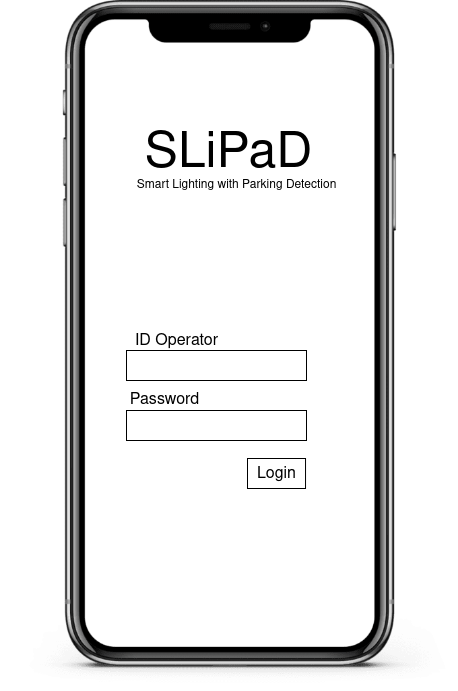
\includegraphics[width=.3\textwidth]{10gui_layouts/App/login}
%	\caption{Mobile Application Layout: Login.}
%	\label{fig:login}
%\end{figure}


%\begin{figure}[H]
%	\centering	
%	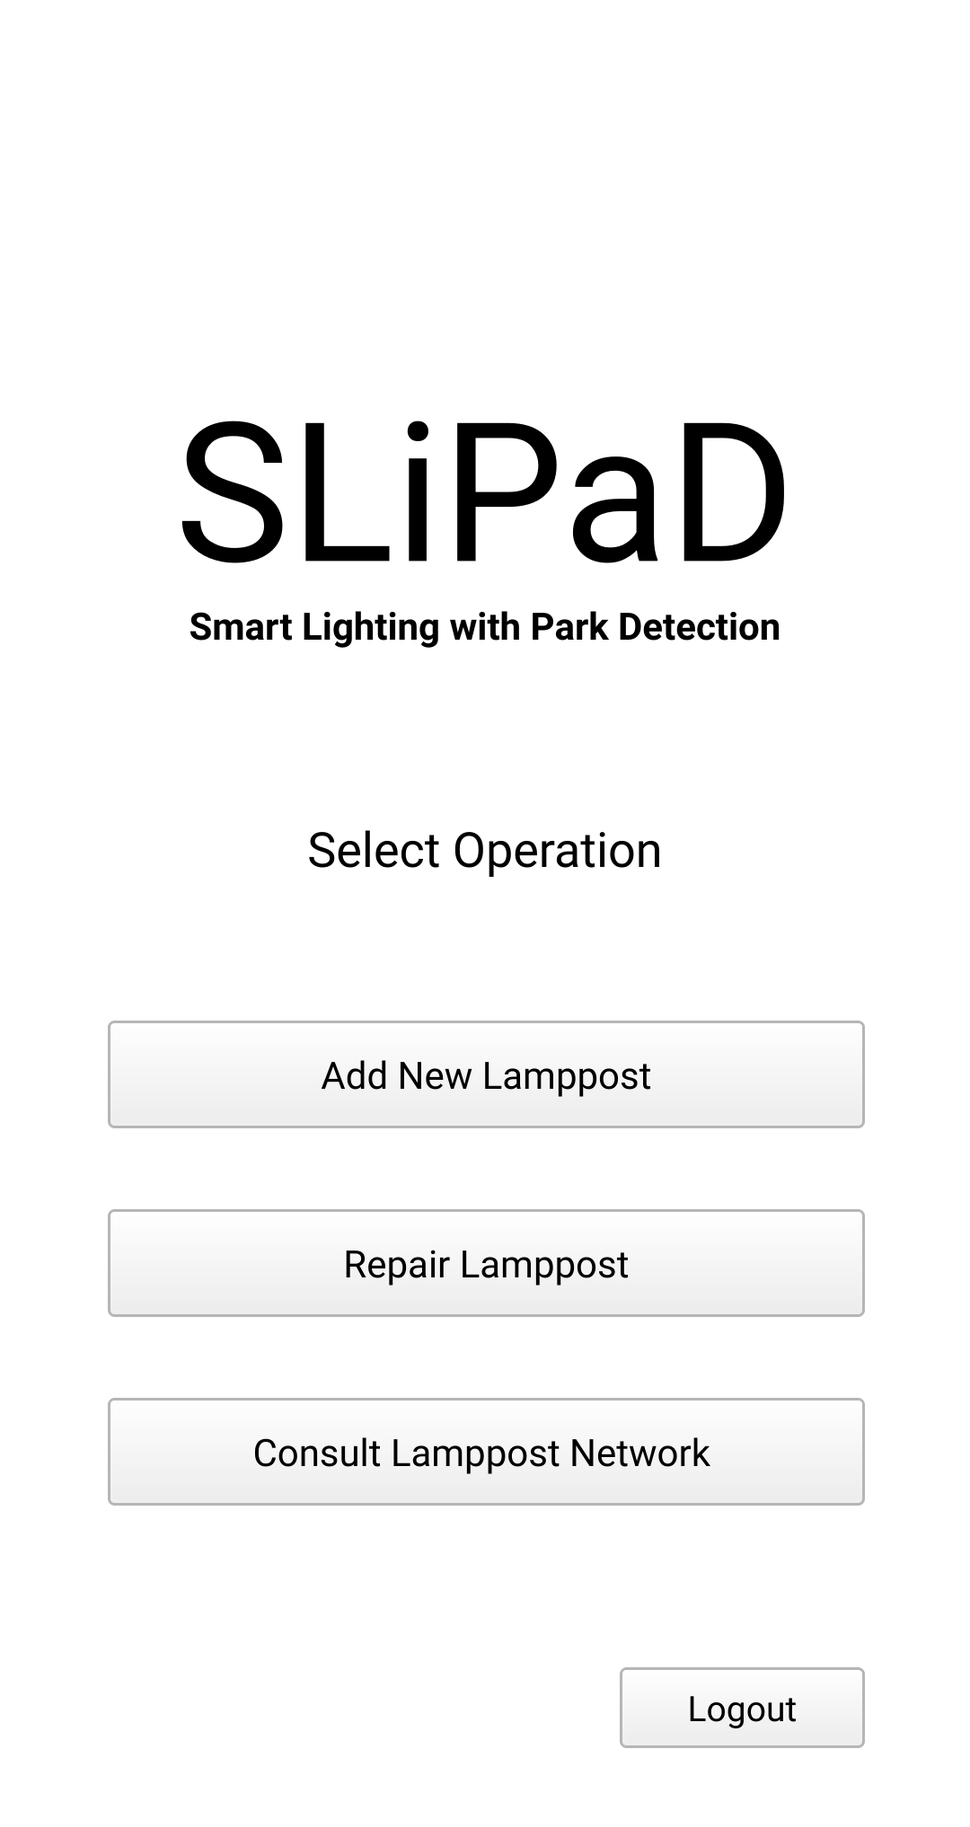
\includegraphics[width=.3\textwidth]{10gui_layouts/App/selectOperation}
%	\caption{Mobile Application Layout: Select Operation.}
%	\label{fig:selectOperation}
%\end{figure}

\begin{figure}[H]
	\centering
	\begin{subfigure}{.5\textwidth}
		\centering
		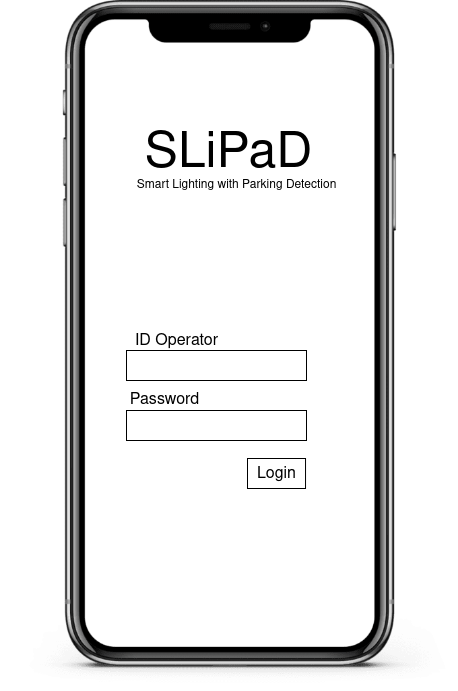
\includegraphics[width=.95\linewidth]{10gui_layouts/App/login}
		\caption{Login.}
		\label{fig:login}
	\end{subfigure}%
	\begin{subfigure}{.5\textwidth}
		\centering
		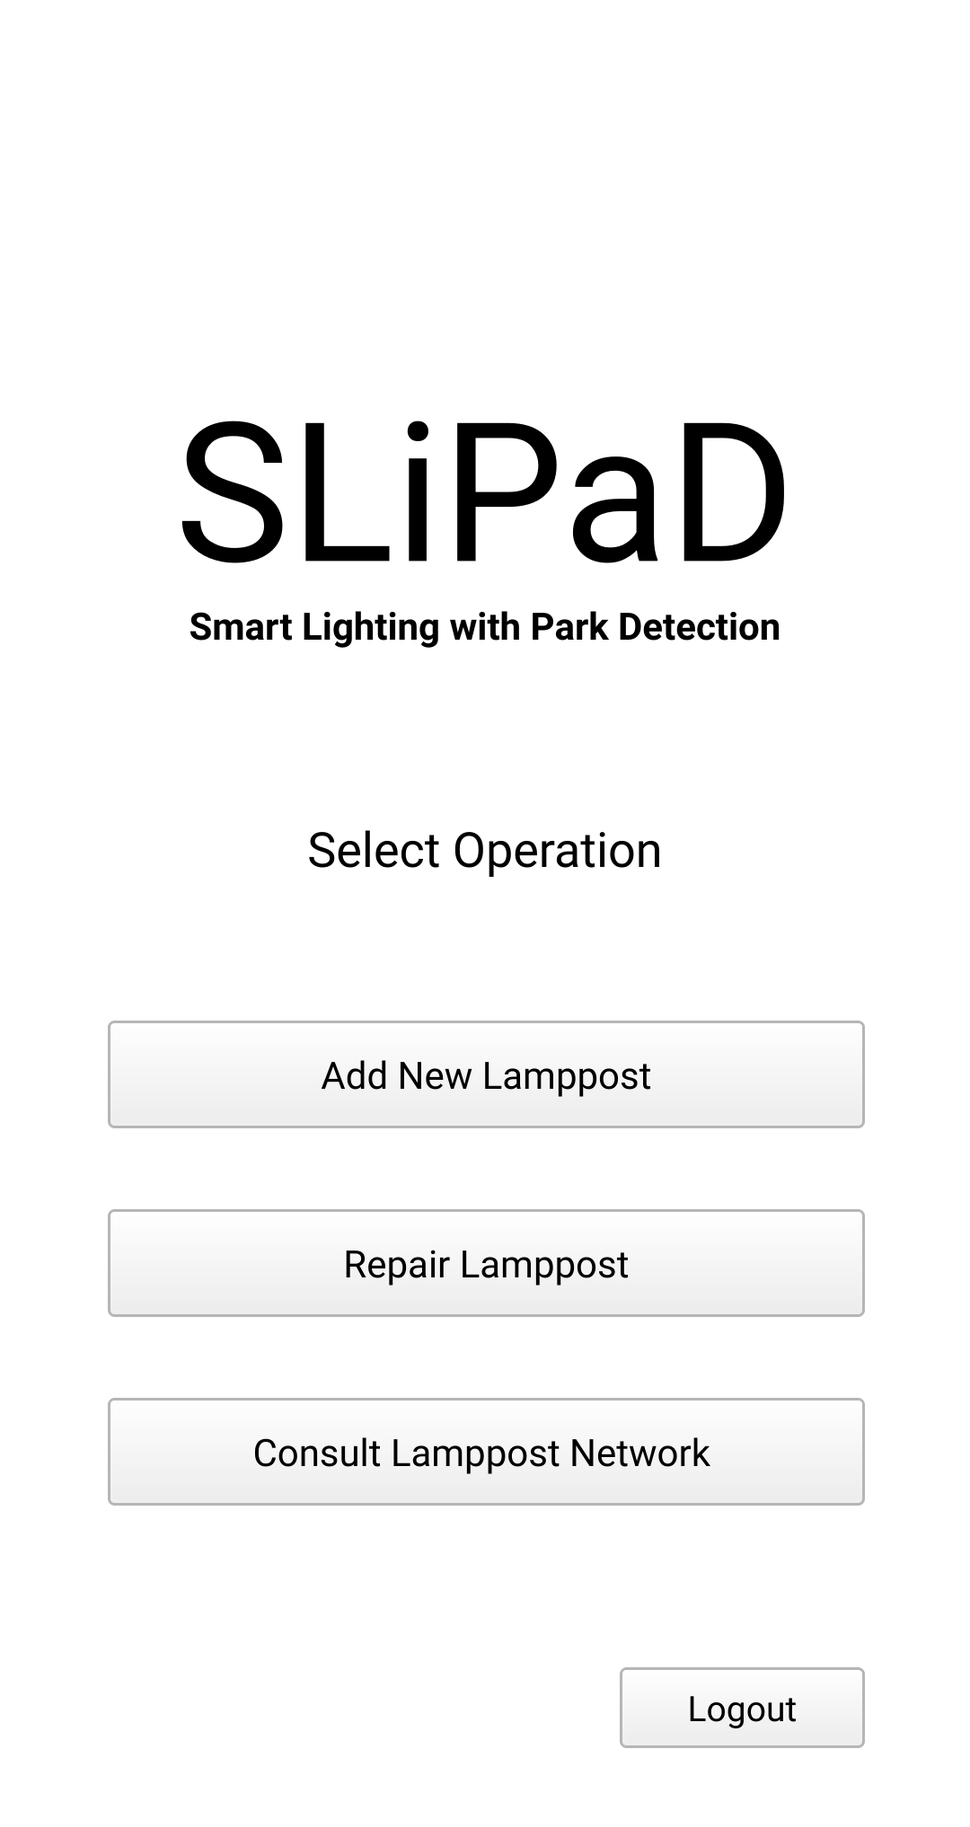
\includegraphics[width=.95\linewidth]{10gui_layouts/App/selectOperation}
		\caption{Select Operation.}
		\label{fig:selectOperation}
	\end{subfigure}
	\caption{Mobile Application Layout.}
	\label{fig:App}
\end{figure}

If the operator clicks on the \textit{Add New Lamppost} option, then he is redirected to the layout represented in figure \ref{fig:addNewLamppost}, where he can add a new lamppost to the network, inserting all the information about the location of the post or use his mobile device actual location. 

\begin{figure}[H]
	\centering	
	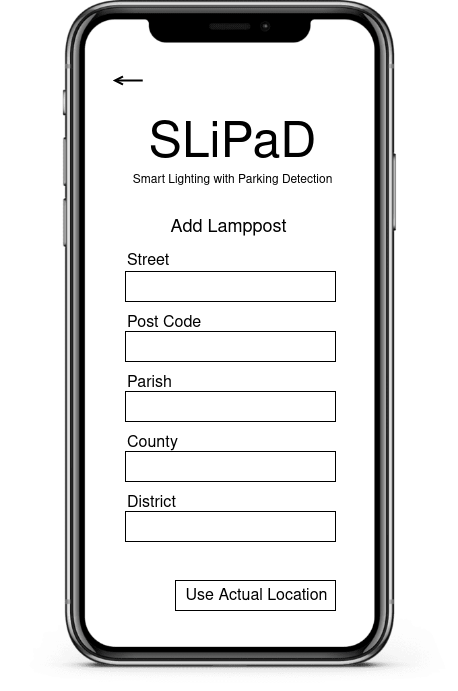
\includegraphics[width=.5\textwidth]{10gui_layouts/App/addNewLamppost}
	\caption{Mobile Application Layout: Add New Lamppost.}
	\label{fig:addNewLamppost}
\end{figure}

\clearpage
If the option chosen was the \textit{Repair Lamppost}, in order to change the lamppost status, he can insert the location of the post or use his mobile device actual location, as seen in figure \ref{fig:repair}.

%\begin{figure}[H]
%	\centering	
%	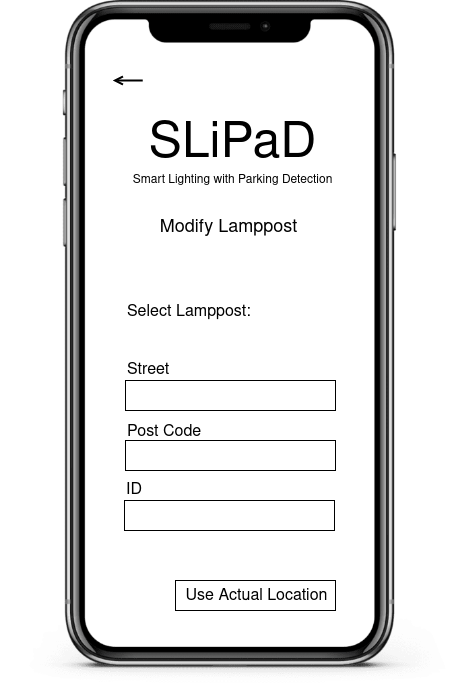
\includegraphics[width=.3\textwidth]{10gui_layouts/App/modifyLamppost}
%	\caption{Mobile Application Layout: Modify Lamppost.}
%	\label{fig:modifyLamppost}
%\end{figure}

If the lamppost selection was valid, then the layout represented in figure \ref{fig:acceptRepair} appears, to the operator confirm that he wants to update the lamppost status.

%\begin{figure}[H]
%	\centering	
%	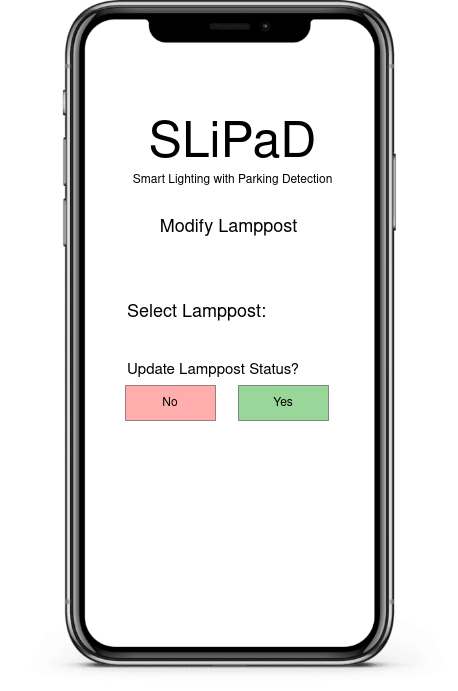
\includegraphics[width=.3\textwidth]{10gui_layouts/App/acceptModify}
%	\caption{Mobile Application Layout: Modify Lamppost Confirmation.}
%	\label{fig:acceptModify}
%\end{figure}

\begin{figure}[H]
	\centering
	\begin{subfigure}{.5\textwidth}
		\centering
		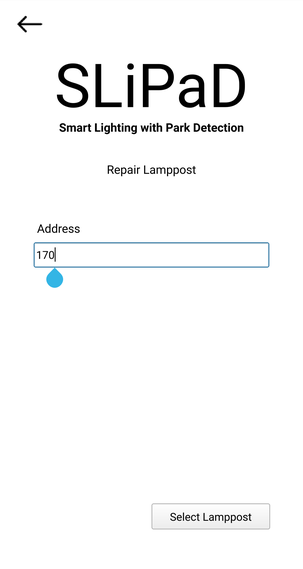
\includegraphics[width=.95\linewidth]{10gui_layouts/App/repair}
		\caption{Repair Lamppost.}
		\label{fig:repair}
	\end{subfigure}%
	\begin{subfigure}{.5\textwidth}
		\centering
		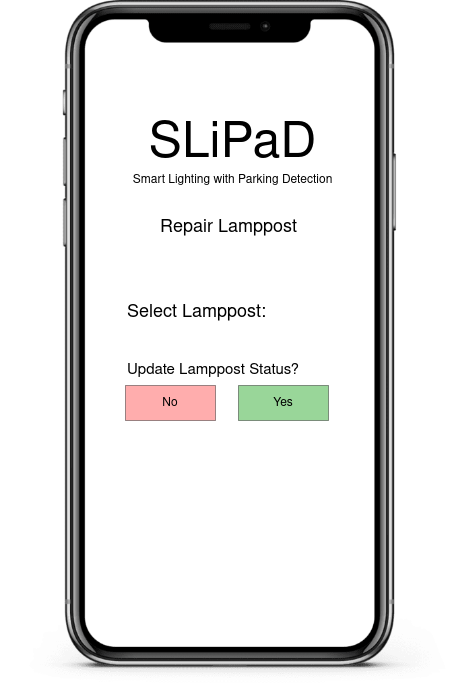
\includegraphics[width=.95\linewidth]{10gui_layouts/App/acceptRepair}
		\caption{Repair Lamppost Confirmation.}
		\label{fig:acceptRepair}
	\end{subfigure}
	\caption{Mobile Application Layout.}
	\label{fig:App2}
\end{figure}

\clearpage
On the other hand, if the operator selects the option \textit{Consult Lamppost Network}, the network information will appear like shown in figure \ref{fig:consultNetwork}, where the red point are lampposts with a broken lamp and the green points are the lampposts with no lamp problems.

\begin{figure}[H]
	\centering	
	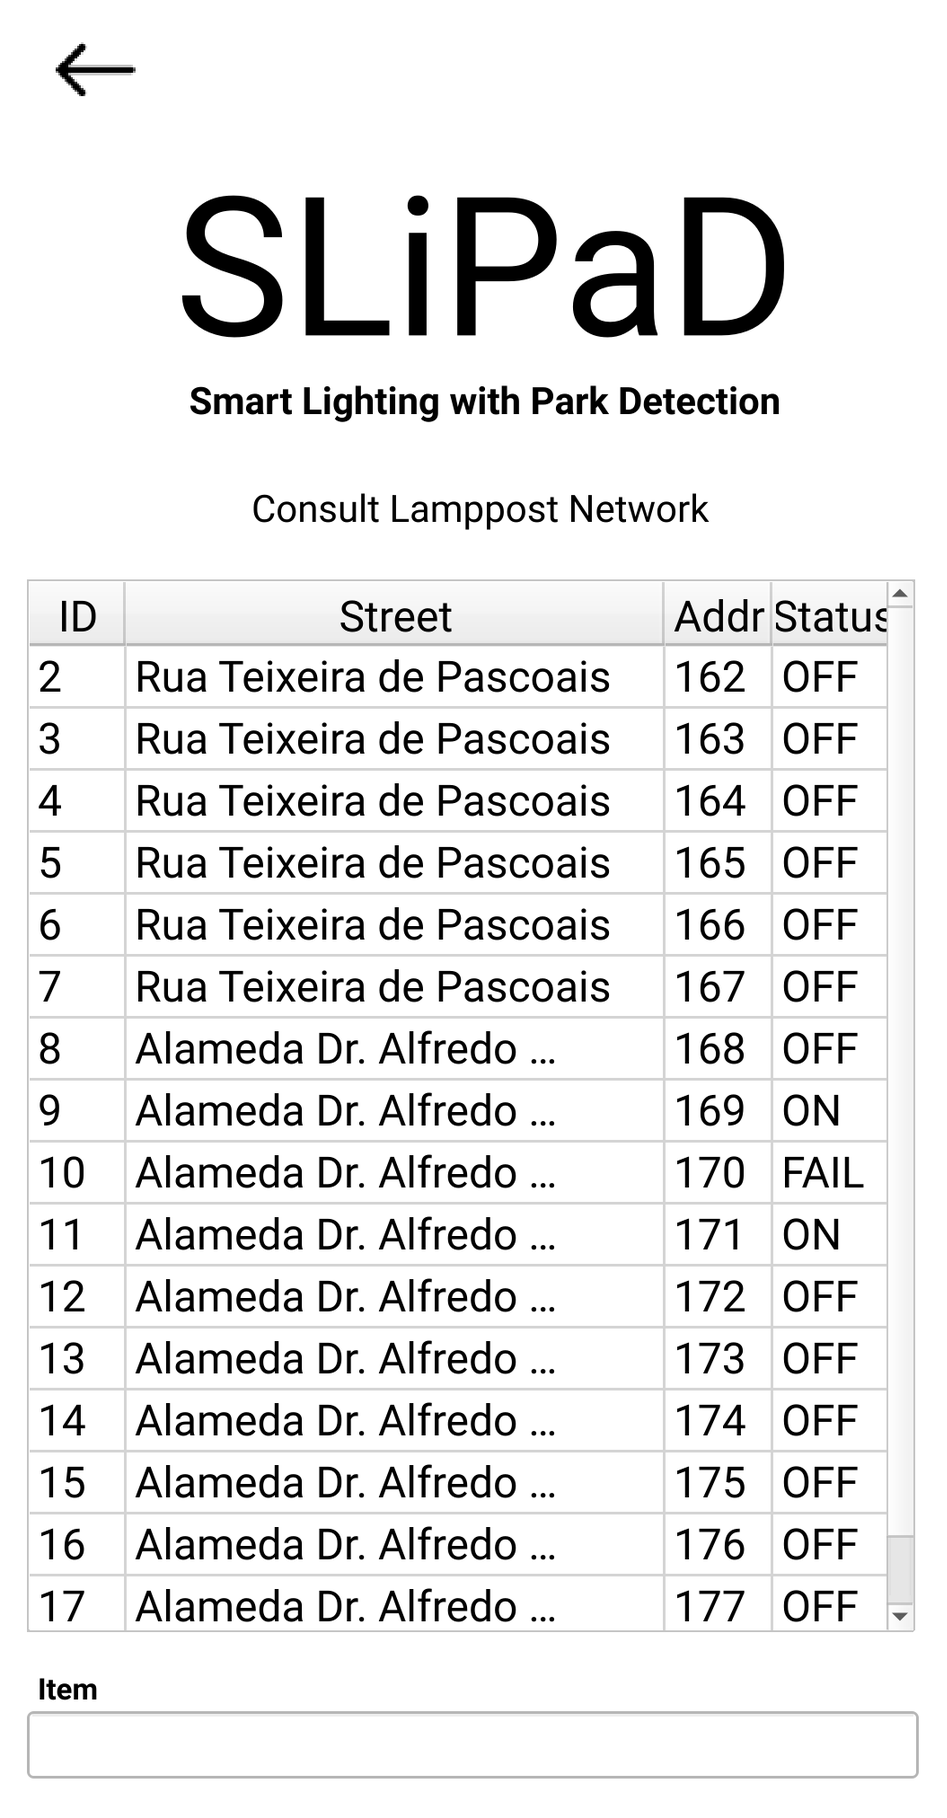
\includegraphics[width=.5\textwidth]{10gui_layouts/App/consultNetwork}
	\caption{Mobile Application Layout: Consult Lamppost Network.}
	\label{fig:consultNetwork}
\end{figure}

\clearpage
\myparagraph{Web Site}

The Web Site can be used by a user that wants to know where there are parking spots available near a location. 

When the user enters the site, it is presented a menu where he can insert the location where he wants to know the parking spots availability or use his actual location, as seen in figure \ref{fig:enterLocation}.

%\begin{figure}[H]
%	\centering	
%	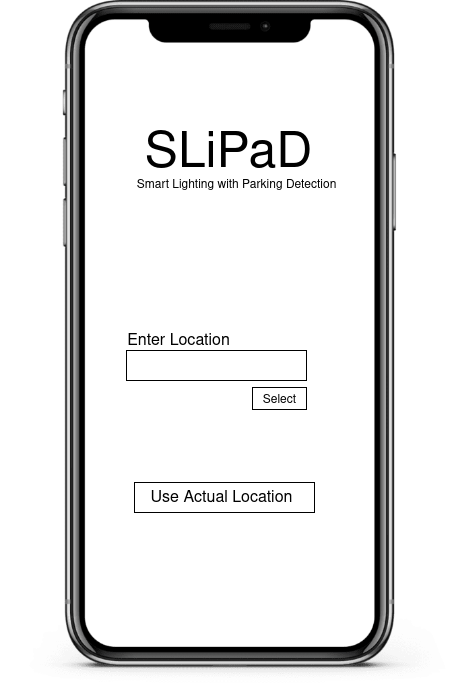
\includegraphics[width=.3\textwidth]{10gui_layouts/WebSite/enterLocation}
%	\caption{Web Site Layout: Enter Location.}
%	\label{fig:enterLocation}
%\end{figure}

After inserting the location, it will be shown the parking spots available near the location inserted, as seen in figure \ref{fig:parksEmpty}, where the red points represent the location of an empty parking spot.

%\begin{figure}[H]
%	\centering	
%	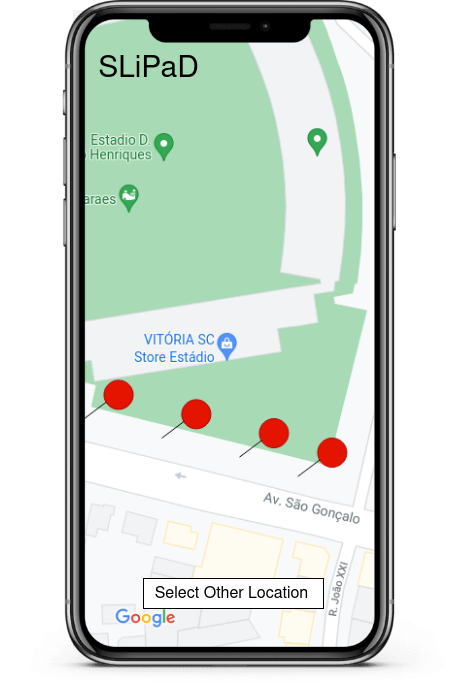
\includegraphics[width=.3\textwidth]{10gui_layouts/WebSite/parksEmpty}
%	\caption{Web Site Layout: Empty Parking Spots Location.}
%	\label{fig:parksEmpty}
%\end{figure}

\begin{figure}[H]
	\centering
	\begin{subfigure}{.5\textwidth}
		\centering
		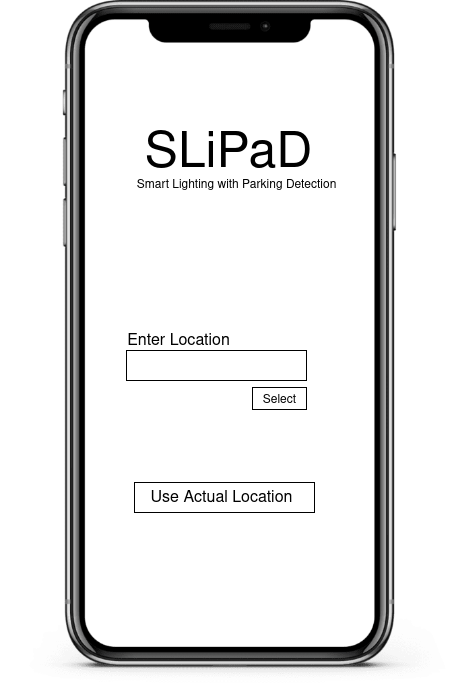
\includegraphics[width=\linewidth]{10gui_layouts/WebSite/enterLocation}
		\caption{Enter Location.}
		\label{fig:enterLocation}
	\end{subfigure}%
	\begin{subfigure}{.5\textwidth}
		\centering
		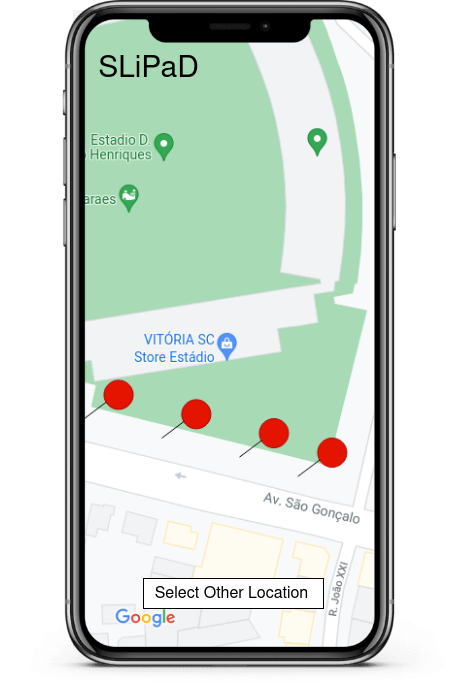
\includegraphics[width=\linewidth]{10gui_layouts/WebSite/parksEmpty}
		\caption{Empty Parking Spots Location.}
		\label{fig:parksEmpty}
	\end{subfigure}
	\caption{Web Site Layout.}
	\label{fig:webSite}
\end{figure}